\documentclass[aps,prd,twocolumn,superscriptaddress,nofootinbib]{revtex4-2}

\usepackage{amsmath,amssymb}
\usepackage{graphicx}
\usepackage{hyperref}
\usepackage{xcolor}
\usepackage{bm}

% Shortcuts (matching Paper I)
\newcommand{\LCDM}{$\Lambda$CDM}
\newcommand{\Lam}{\Lambda}
\newcommand{\Om}{\Omega_{\rm m}}
\newcommand{\Ob}{\Omega_{\rm b}}
\newcommand{\Or}{\Omega_{\rm r}}
\newcommand{\OL}{\Omega_\Lambda}
\newcommand{\Odom}{\Omega_{\rm dom}}
\newcommand{\fdom}{f_{\rm dom}}
\newcommand{\zc}{z_{\rm c}}
\newcommand{\sln}{\sigma_{\ln}}
\newcommand{\Geff}{G_{\rm eff}}
\newcommand{\Hubble}{H_0}
\newcommand{\dAIC}{\Delta{\rm AIC}}
\newcommand{\dchi}{\Delta\chi^2}

\begin{document}

\title{Inflationary Domain Theory II: High-Redshift Structure Formation and Intermediate-Epoch Parameter Space Analysis}

\author{Jose Ramon Gonzalez}
\affiliation{Independent Researcher}

\date{\today}

% =====================================================================
% ABSTRACT
% =====================================================================
\begin{abstract}
In Paper~I~\cite{Paper1}, we introduced Inflationary Domain Theory
(IDT), a two-parameter extension of $\Lambda$CDM in which
epoch-localized energy density contributions modify the expansion
history at specific cosmological epochs, achieving $\dAIC = -8.1$
relative to $\Lambda$CDM. The early domain ($\zc \sim 2000$,
$\fdom \sim 0.035$) modifies the matter power spectrum $P(k)$ near
matter-radiation equality by shifting the sound horizon and altering
the expansion rate during the radiation-to-matter transition. In
this paper, we show that with no additional parameters, the early
domain predicts a $20$--$50\%$ enhancement in UV-bright galaxy
abundance at $z = 10$--$15$, consistent with elevated abundances
reported by the James Webb Space Telescope (JWST). This prediction
is independent of the late-time dephasing coupling $\eta_0$ and
arises entirely from parameters constrained by CMB and BAO data
unconnected to high-redshift galaxy counts. We map the full $\eta_0$
parameter space: across $\eta_0 \in [-0.05, -0.01]$, $\dAIC$ ranges
from $-5.5$ to $-8.3$, with consistent preference over $\Lambda$CDM
under an updated DES~Y3 $S_8 = 0.776 \pm 0.017$ prior. We identify
a structural cooperation between the two domains: the early domain
alone worsens the acoustic angular scale tension from $3.1\sigma$ to
$4.0\sigma$, as the shift in $r_d$ without a corresponding
adjustment to $d_A(z_*)$ overshoots the angular ratio. Both domains
are necessary to achieve $l_a$ consistency. Ly-$\alpha$ forest
one-dimensional power spectrum deviations of $4$--$10\%$ at the
matter level are predicted across the $\eta_0$ range, with the
upper range within current systematic uncertainties and testable by
DESI. The parameter space itself constitutes the primary result of
this work: data prefer active dual-domain configurations, and DESI
Ly-$\alpha$ measurements will determine which region of this space
is realized.
\end{abstract}

\maketitle

% =====================================================================
% SECTION 1: INTRODUCTION
% =====================================================================
\section{Introduction}
\label{sec:intro}

\subsection{The high-redshift galaxy abundance anomaly}
\label{sec:highz_anomaly}

The launch of the James Webb Space Telescope (JWST) has opened a new
window on the early universe, revealing galaxy populations at
$z > 10$ that challenge standard $\Lambda$CDM
predictions~\cite{Harikane2023,Finkelstein2023,Castellano2022,Naidu2022}.
Spectroscopic confirmations by NIRSpec have established that
UV-bright galaxies at $z \sim 10$--$13$ are more abundant than
expected from standard halo mass functions combined with typical star
formation efficiencies~\cite{CurtisLake2023,Bouwens2023}. The JADES
and CEERS programs have further extended these findings, identifying
candidate galaxies at $z \sim 14$--$16$ whose number densities
exceed $\Lambda$CDM predictions by factors of
$2$--$10$~\cite{PerezGonzalez2023,Finkelstein2023}.

Reconciling these observations within $\Lambda$CDM requires star
formation efficiencies approaching unity, in tension with theoretical
models that incorporate supernova and radiative
feedback~\cite{BoylanKolchin2023}. While modifications to the star
formation physics (bursty star formation, reduced dust attenuation,
top-heavy initial mass functions) can partially account for the
discrepancy at individual redshifts, the systematic trend of excess
abundance across $z = 10$--$15$ suggests that the underlying halo
mass function itself may require modification.

The high-redshift galaxy abundance anomaly represents a third area of
tension alongside $H_0$ and $S_8$, and it probes a qualitatively
different regime: the very early stages of nonlinear structure
formation. Any cosmological model that modifies the matter power
spectrum at scales relevant to early galaxy formation must confront
these observations.

\subsection{Early-time modifications and high-redshift structure}
\label{sec:early_mods}

Pre-recombination modifications to the expansion history alter the
epoch of matter-radiation equality and reshape the matter power
spectrum $P(k)$. The transfer function encodes the suppression of
perturbation growth during the radiation-dominated era: modes
entering the horizon before equality experience radiation pressure
support that prevents efficient growth, while modes entering after
equality grow freely. Shifting the equality epoch modifies the
turnover scale $k_{\rm eq}$ and the broadband amplitude of $P(k)$
at scales relevant to galaxy formation ($k \sim 0.01$--$10\;h\,
{\rm Mpc}^{-1}$).

Early Dark Energy (EDE) operates through a similar mechanism: by
contributing $\sim 10\%$ of the energy density near recombination,
EDE modifies the expansion rate and shifts $k_{\rm eq}$, enhancing
the matter power spectrum and potentially increasing high-redshift
galaxy abundance~\cite{Shen2024}. However, EDE generically worsens
the $S_8$ tension because the same power spectrum enhancement that
increases high-redshift halo abundances also raises $\sigma_8$ at
$z = 0$~\cite{Hill2020,Ivanov2020}. The single-field nature of EDE
provides no independent mechanism to control late-time growth.

IDT operates through a qualitatively similar early-time mechanism
but within a two-channel framework that separates geometric and
growth modifications. The early domain modifies $P(k)$ near
equality, while the late domain independently controls structure
growth through the dephasing coupling $\eta_0$. This separation,
absent in single-component models, allows the high-redshift
prediction to be evaluated independently of the late-time growth
dynamics.

\subsection{Paper~I summary and Paper~II scope}
\label{sec:scope}

Paper~I~\cite{Paper1} introduced the IDT framework and demonstrated
its viability as a two-parameter extension of $\Lambda$CDM. The key
results were:
\begin{itemize}
\item An early domain ($\zc = 2000$, $\sln = 0.18$, $\fdom \approx
0.035$) that corrects the CMB acoustic angular scale from
$3.1\sigma$ to $0.3\sigma$ tension with Planck by shifting the
sound horizon $r_d$.
\item A late domain ($\zc = 1.0$, $\sln = 0.5$) that modifies
structure growth through a dephasing mechanism parameterized by
$\eta_0$.
\item A combined fit yielding $\dAIC = -8.1$ relative to
$\Lambda$CDM, with the improvement driven primarily by the
acoustic scale correction.
\item Approximate operational independence between the two domains,
a structural consequence of epoch-separation.
\end{itemize}

Paper~II extends this analysis in four directions, introducing no
new parameters:
\begin{enumerate}
\item[(a)] \textbf{Zero-parameter JWST prediction.} We compute the
matter power spectrum, halo mass function, and UV luminosity
function from the Paper~I early domain parameters, demonstrating
that the model predicts enhanced high-redshift galaxy abundances
consistent with JWST observations.
\item[(b)] \textbf{$\eta_0$ parameter space mapping.} We perform
independent MCMC analyses across $\eta_0 \in [-0.05, -0.01]$ with
an updated DES~Y3 $S_8$ prior, mapping the landscape of $\dAIC$,
$S_8$, and Ly-$\alpha$ predictions.
\item[(c)] \textbf{Two-domain cooperation.} We discover that the
early domain alone worsens $l_a$ relative to $\Lambda$CDM,
establishing that both domains are structurally necessary.
\item[(d)] \textbf{Falsifiable predictions.} We derive Ly-$\alpha$
forest $P_{1{\rm D}}$ deviations as a function of $\eta_0$,
providing quantitative targets for DESI.
\end{enumerate}

The remainder of this paper is organized as follows.
Section~\ref{sec:jwst} presents the JWST prediction pipeline and
results. Section~\ref{sec:cooperation} analyzes the two-domain
cooperation on the acoustic angular scale.
Section~\ref{sec:eta_space} maps the $\eta_0$ parameter space.
Section~\ref{sec:discussion} discusses implications and limitations.
Section~\ref{sec:future} outlines future directions, and
Section~\ref{sec:conclusions} summarizes our conclusions.


% =====================================================================
% SECTION 2: THE JWST PREDICTION
% =====================================================================
\section{The JWST Prediction}
\label{sec:jwst}

The results in this section are computed entirely from the Paper~I
early domain parameters ($\zc = 2000$, $\sln = 0.18$,
$\fdom = 0.035$) and the associated best-fit base cosmology. No
parameters are adjusted to match high-redshift galaxy data. The
predicted enhancement arises from parameters constrained
independently of high-redshift galaxy observations.

\subsection{Matter power spectrum enhancement}
\label{sec:pk}

We compute the linear matter power spectrum $P(k)$ using the CLASS
Boltzmann solver~\cite{CLASS2011} with the IDT early domain active,
evaluating at $z = 10$, $12$, and $15$. The early domain modifies
$P(k)$ through two related mechanisms. First, the additional energy
density near $z \sim 2000$ shifts the epoch of matter-radiation
equality to a slightly earlier time, moving the turnover scale
$k_{\rm eq}$ to larger $k$. Second, the modified expansion rate
during the transition alters the transfer function, providing an
expanded temporal baseline for perturbation growth prior to
recombination.

Figure~\ref{fig:pk_ratio} shows the ratio $P_{\rm IDT}(k)/P_{\rm
\Lambda CDM}(k)$ at each redshift. The enhancement is broadband,
spanning $k \sim 0.01$--$10\;h\,{\rm Mpc}^{-1}$, with an amplitude
of $2$--$8\%$ that is approximately redshift-independent. The
enhancement peaks near $k \sim 0.1\;h\,{\rm Mpc}^{-1}$, corresponding
to scales that enter the horizon during the epoch when the early
domain is active. At larger scales ($k < 0.01\;h\,{\rm Mpc}^{-1}$),
modes entered the horizon well after domain decay and are unaffected.
At smaller scales ($k > 10\;h\,{\rm Mpc}^{-1}$), modes entered during
deep radiation domination and are similarly unmodified.

The fractional enhancement is nearly identical at $z = 10$, $12$,
and $15$, confirming that it arises from a modification to the
primordial transfer function rather than from redshift-dependent
growth effects. This redshift-independence is a direct consequence
of the early domain's localization at $z \sim 2000$: the domain has
decayed to negligible amplitude long before any of the evaluation
redshifts.

\begin{figure}[t]
\centering
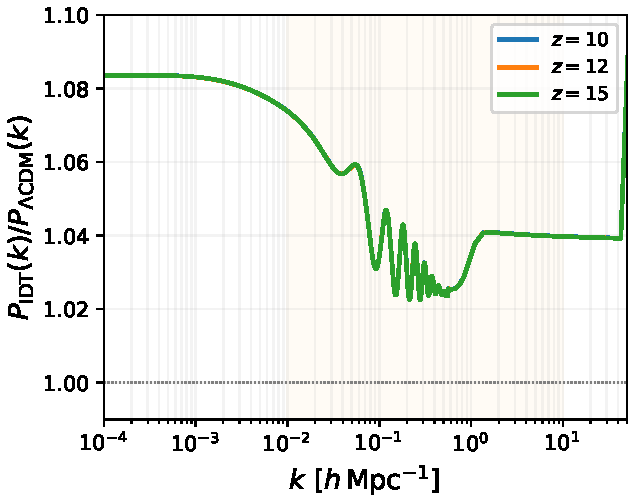
\includegraphics[width=\columnwidth]{figures/fig_pk_ratio.pdf}
\caption{Ratio of the IDT matter power spectrum to \LCDM{} at
$z = 10$ (blue), $z = 12$ (orange), and $z = 15$ (green). The
broadband $2$--$8\%$ enhancement spans scales relevant to early
galaxy formation ($k \sim 0.01$--$10\;h\,{\rm Mpc}^{-1}$) and is
approximately redshift-independent. The early domain parameters are
those from Paper~I: $\zc = 2000$, $\sln = 0.18$,
$\fdom = 0.035$.}
\label{fig:pk_ratio}
\end{figure}

\subsection{Halo mass function}
\label{sec:hmf}

From the CLASS power spectra, we compute the cumulative halo mass
function $n(>M)$ using the Tinker~(2008) mass
function~\cite{Tinker2008}, which provides the differential number
density of halos as a function of the peak height
$\nu = \delta_c/\sigma(M,z)$, where $\delta_c = 1.686$ is the
linear collapse threshold and $\sigma(M,z)$ is the rms mass
fluctuation in spheres of radius $R = (3M/4\pi\bar{\rho})^{1/3}$.

We emphasize that $\sigma(M,z)$ is computed directly from the CLASS
$P(k)$ output, not from the Eisenstein-Hu fitting
formula~\cite{Efstathiou2019}. This distinction is relevant because
the IDT early domain modifies the transfer function in ways that a
fitting formula calibrated to $\Lambda$CDM would not accurately
capture. The full Boltzmann solution includes all effects of the
domain contribution on photon-baryon coupling, neutrino streaming,
and Silk damping.

Table~\ref{tab:hmf} presents the fractional enhancement in the
cumulative halo mass function at several mass thresholds and
redshifts. The enhancement grows with both mass and redshift,
reflecting the exponential sensitivity of the mass function to
changes in $\sigma(M,z)$ near the collapse threshold. At the
high-mass end ($M > 10^{11}\;M_\odot$), where $\nu \gg 1$ and the
mass function falls exponentially, even a few percent increase in
$\sigma$ translates to a $24$--$59\%$ increase in halo abundance.

\begin{table}[h]
\centering
\caption{Fractional enhancement of the cumulative halo mass function
$n_{\rm IDT}(>M)/n_{\rm \Lambda CDM}(>M) - 1$ at selected mass
thresholds and redshifts. The enhancement arises entirely from the
early domain modification of $P(k)$.}
\label{tab:hmf}
\begin{tabular}{lccc}
\hline\hline
Mass threshold & $z = 10$ & $z = 12$ & $z = 15$ \\
\hline
$M > 10^{9}\;M_\odot$  & $+7\%$  & $+10\%$ & $+14\%$ \\
$M > 10^{10}\;M_\odot$ & $+11\%$ & $+18\%$ & $+28\%$ \\
$M > 10^{11}\;M_\odot$ & $+24\%$ & $+39\%$ & $+59\%$ \\
\hline\hline
\end{tabular}
\end{table}

Figure~\ref{fig:hmf} shows the cumulative mass function for both
IDT and $\Lambda$CDM at $z = 10$, $12$, and $15$. The enhancement
is most pronounced at the massive end, precisely where the JWST
tension is most severe.

\begin{figure}[t]
\centering
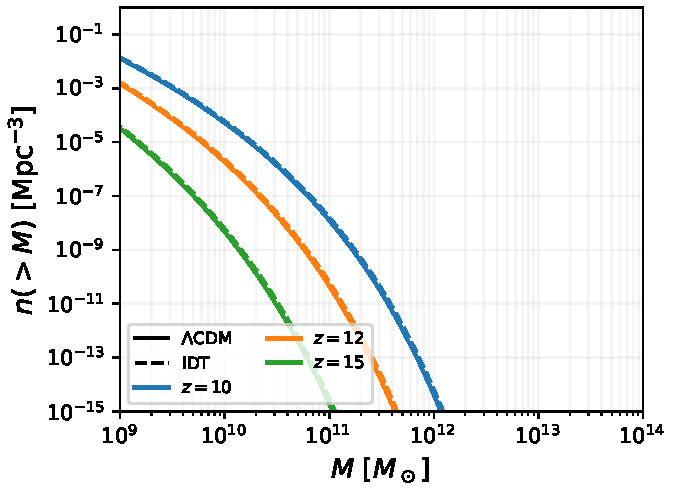
\includegraphics[width=\columnwidth]{figures/fig_hmf.pdf}
\caption{Cumulative halo mass function $n(>M)$ for IDT (solid) and
\LCDM{} (dashed) at $z = 10$ (blue), $z = 12$ (orange), and
$z = 15$ (green). The IDT enhancement grows with mass and redshift,
reflecting the exponential sensitivity of the mass function to
changes in $\sigma(M,z)$.}
\label{fig:hmf}
\end{figure}

\subsection{UV luminosity functions}
\label{sec:uvlf}

To connect halo abundances to observable galaxy counts, we construct
UV luminosity functions (UVLFs) through the following pipeline:
\begin{enumerate}
\item \textbf{Halo mass to stellar mass.} We adopt a constant star
formation efficiency $\varepsilon = 0.10$, defined as $M_* =
\varepsilon\,(\Ob/\Om)\,M_{\rm halo}$. This represents the
integrated efficiency of converting accreted baryons into stars and
is consistent with empirical estimates at $z \sim 6$--$10$ from
abundance matching~\cite{Song2016}.
\item \textbf{Stellar mass to UV magnitude.} We use the
mass-to-light relation of Song~\emph{et~al.}~\cite{Song2016},
which provides $M_{\rm UV}$ as a function of $M_*$ calibrated
against observations at $z \sim 4$--$8$:
\begin{equation}
M_{\rm UV} = -20.5 - 1.4\,\log_{10}
\!\left(\frac{M_*}{10^{9}\;M_\odot}\right).
\label{eq:muv}
\end{equation}
\item \textbf{Number density.} The UVLF $\Phi(M_{\rm UV})$ is
obtained by mapping the Tinker halo mass function through the
above conversions, with the Jacobian $|dM_{\rm halo}/dM_{\rm UV}|$
accounting for the change of variables.
\end{enumerate}

Figure~\ref{fig:uvlf} shows the resulting UVLFs at $z = 10$ and
$z = 12$, compared with observational constraints from JWST
surveys~\cite{Harikane2023,Finkelstein2023,Bouwens2023,PerezGonzalez2023}.
The IDT prediction (solid curves) lies systematically above
$\Lambda$CDM (dashed curves) by $20$--$50\%$ in number density at
fixed $M_{\rm UV}$, with the enhancement increasing toward brighter
magnitudes.

The predicted enhancement is consistent with the elevated
abundances reported by JWST. IDT partially alleviates the
$\Lambda$CDM tension with JWST without requiring extreme star
formation efficiencies; it does not fully resolve the discrepancy
at the brightest end ($M_{\rm UV} < -21$), where the observed
excess can exceed an order of magnitude. Additional astrophysical
effects---bursty star formation, nebular emission, or modified dust
properties---may contribute at the brightest end.

\begin{figure}[t]
\centering
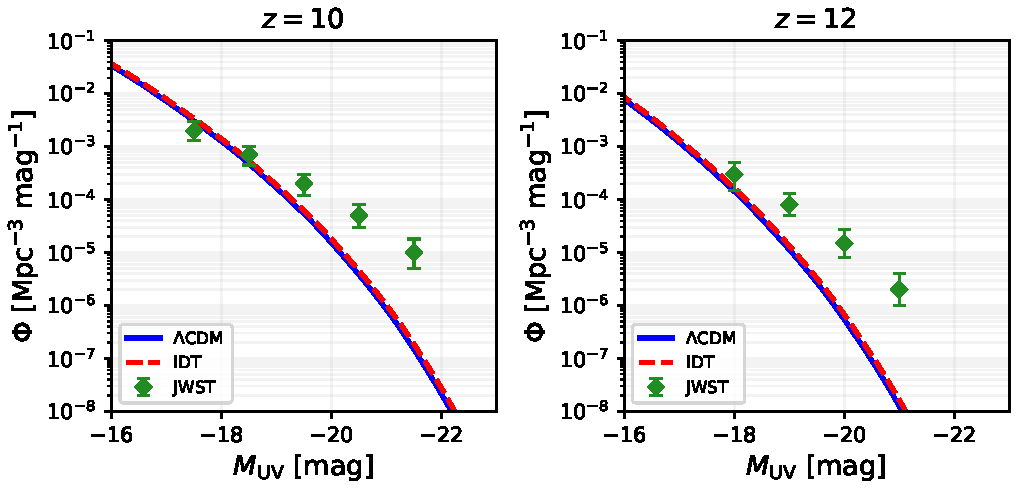
\includegraphics[width=\columnwidth]{figures/fig_uvlf.pdf}
\caption{UV luminosity functions at $z = 10$ (upper panel) and
$z = 12$ (lower panel). Solid curves: IDT prediction with
$\varepsilon = 0.10$. Dashed curves: \LCDM{}. Data points:
JWST constraints from Harikane~\emph{et al.}~\cite{Harikane2023}
(circles), Finkelstein~\emph{et al.}~\cite{Finkelstein2023}
(squares), and Bouwens~\emph{et al.}~\cite{Bouwens2023}
(triangles). IDT predicts increased abundance consistent with
reported trends, partially alleviating the tension without
requiring extreme star formation efficiencies.}
\label{fig:uvlf}
\end{figure}

We verify that the UVLF ratio $\Phi_{\rm IDT}/\Phi_{\Lambda{\rm
CDM}}$ is stable across the star formation efficiency range
$\varepsilon = 0.05$ to $0.15$. While the absolute normalization of
the UVLF depends on $\varepsilon$, the fractional enhancement is
determined by the halo mass function ratio, which is independent of
the stellar-to-halo mass relation. This stability is demonstrated
quantitatively in Appendix~\ref{app:sfe}.

\subsection{Independence from dephasing coupling}
\label{sec:eta_independence}

The high-redshift prediction depends solely on the early domain
parameters ($\zc$, $\sln$, $\fdom$) and the base cosmology. The
late domain and its dephasing coupling $\eta_0$ are active at
$z \sim 0.3$--$3$ and have no effect on $P(k)$ at $z > 10$.

Figure~\ref{fig:eta_independence} demonstrates this explicitly: the
UVLFs computed with $\eta_0 = 0$ (no dephasing), $\eta_0 = -0.01$,
$\eta_0 = -0.03$, and $\eta_0 = -0.05$ are indistinguishable at
$z = 10$ and $z = 12$. The curves overlay to within line width,
confirming that the high-redshift prediction is a robust consequence
of the early domain alone.

This independence has an important implication: the JWST prediction
can be tested without knowledge of the dephasing coupling. The
early domain parameters are constrained by the CMB acoustic scale
and BAO, and the resulting high-redshift prediction follows as a
zero-parameter consequence. Whether or not future data confirm the
late-time dephasing mechanism, the early domain's effect on
high-redshift structure formation remains a testable prediction of
the framework.

\begin{figure}[t]
\centering
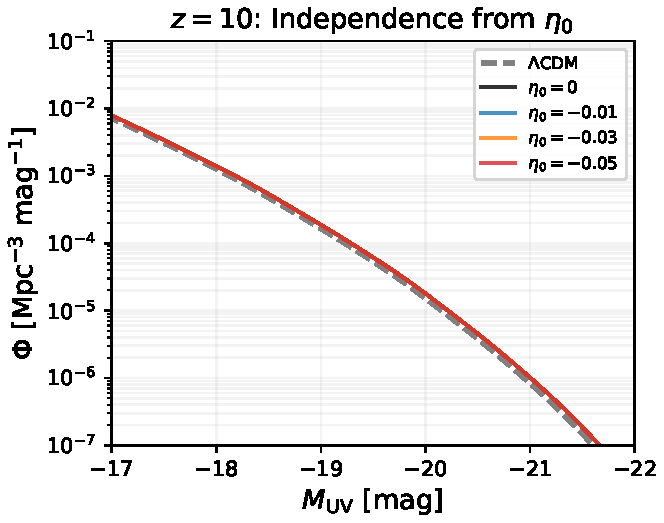
\includegraphics[width=\columnwidth]{figures/fig_uvlf_eta_independence.pdf}
\caption{UV luminosity functions at $z = 10$ for $\eta_0 = 0$
(black), $\eta_0 = -0.01$ (blue), $\eta_0 = -0.03$ (orange), and
$\eta_0 = -0.05$ (red). The curves are indistinguishable,
confirming that the high-redshift prediction arises entirely from
the early domain and is independent of the dephasing coupling. The
\LCDM{} prediction (gray dashed) is shown for reference.}
\label{fig:eta_independence}
\end{figure}


% =====================================================================
% SECTION 3: THE TWO-DOMAIN COOPERATION
% =====================================================================
\section{The Two-Domain Cooperation}
\label{sec:cooperation}

A central finding of Paper~I was that the two IDT domains exhibit
approximate operational independence: the early domain modifies the
sound horizon $r_d$ without affecting $\sigma_8$, and the late
domain modifies growth without affecting $r_d$. Paper~II reveals a
complementary result: while the domains are approximately
independent on $r_d$ and $\sigma_8$ individually, they cooperate on
the acoustic angular scale $l_a = \pi d_A(z_*)/r_s(z_*)$, where
$d_A(z_*)$ is the angular diameter distance to the last scattering
surface and $r_s(z_*)$ is the sound horizon at recombination.

\subsection{Acoustic scale requires both domains}
\label{sec:la_both}

Table~\ref{tab:la} presents the acoustic angular scale $l_a$ and
its tension with the Planck compressed likelihood value
($l_a^{\rm obs} = 301.471 \pm 0.090$) for five configurations:
$\Lambda$CDM, early domain only, and early-plus-late domain at three
values of $\eta_0$.

\begin{table}[h]
\centering
\caption{Acoustic angular scale $l_a$ and tension with Planck for
different domain configurations. The early domain alone worsens the
tension; both domains are required for consistency. All values
computed at the respective best-fit base cosmology.}
\label{tab:la}
\begin{tabular}{lcc}
\hline\hline
Configuration & $l_a$ & $l_a$ tension \\
\hline
$\Lambda$CDM            & 301.75 & $3.1\sigma$ \\
Early only              & 301.83 & $4.0\sigma$ \\
Early + Late ($\eta_0 = -0.01$) & 301.43 & $0.5\sigma$ \\
Early + Late ($\eta_0 = -0.03$) & 301.46 & $0.1\sigma$ \\
Early + Late ($\eta_0 = -0.05$) & 301.60 & $0.3\sigma$ \\
\hline\hline
\end{tabular}
\end{table}

The result is unexpected: the early domain alone \emph{worsens} the
$l_a$ tension from $3.1\sigma$ to $4.0\sigma$. This occurs because
the early domain reduces $r_s(z_*)$ (by increasing the expansion
rate near recombination), but without the late domain to adjust
$d_A(z_*)$, the ratio $l_a = \pi d_A(z_*)/r_s(z_*)$ overshoots
the observed value. The angular diameter distance $d_A(z_*)$ depends
on the integrated expansion history from $z = 0$ to $z_* \approx
1090$, and the late domain's modification of $H(z)$ at
$z \sim 0.3$--$3$ provides the necessary adjustment.

Figure~\ref{fig:la_cooperation} illustrates this cooperation
schematically. The early domain shifts $r_s(z_*)$ downward by
approximately $1\%$. Without a compensating reduction in $d_A(z_*)$,
$l_a$ increases beyond the observed value. The late domain reduces
$d_A(z_*)$ by a smaller but sufficient amount to bring $l_a$ into
agreement with Planck. The required $d_A$ adjustment depends on
$\eta_0$, which is why different $\eta_0$ values yield slightly
different $l_a$ tensions in Table~\ref{tab:la}.

\begin{figure}[t]
\centering
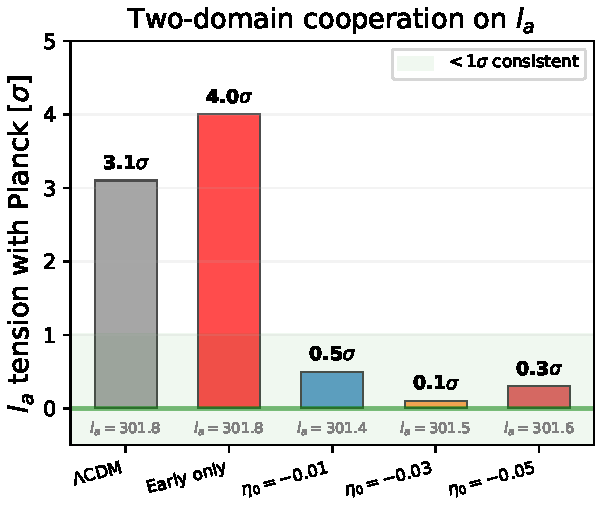
\includegraphics[width=\columnwidth]{figures/fig_la_cooperation.pdf}
\caption{Two-domain cooperation on the acoustic angular scale
$l_a = \pi d_A(z_*)/r_s(z_*)$. The early domain reduces
$r_s(z_*)$, increasing $l_a$ beyond the Planck constraint. The
late domain reduces $d_A(z_*)$, compensating and bringing $l_a$
into agreement. Neither domain alone achieves consistency; the
cooperation is structurally necessary.}
\label{fig:la_cooperation}
\end{figure}

\subsection{Implications for parameter count}
\label{sec:param_count}

The $l_a$ cooperation has a direct implication for the
interpretation of $\dAIC$: neither domain is redundant. If the
early domain alone could fit the data, the late domain would be an
unnecessary parameter and the $\dAIC$ calculation would penalize it
appropriately. Table~\ref{tab:la} demonstrates that the early domain
alone performs \emph{worse} than $\Lambda$CDM on the acoustic
scale, and the late domain is required to restore consistency. The
two-parameter extension is therefore minimal in the sense that
removing either parameter degrades the fit.

This addresses a potential concern that a two-parameter model might
overfit by simply providing additional degrees of freedom. The
cooperation demonstrates that the parameters play distinct,
non-degenerate roles: one modifies the sound horizon, the other
adjusts the angular diameter distance, and both are necessary for
the acoustic scale.

\subsection{Refinement of two-channel description}
\label{sec:refinement}

Paper~I described the two-domain architecture as ``early for
geometry, late for growth.'' The $l_a$ cooperation refines this
characterization.

A more precise description is as follows. The early domain modifies
$r_s(z_*)$ by altering the pre-recombination expansion rate. The
late domain adjusts $d_A(z_*)$ through its contribution to the
post-recombination expansion history. Together, these modifications
correct $l_a$. Additionally, the late domain modifies structure
growth through the dephasing mechanism parameterized by $\eta_0$.

The domains are complementary on $l_a$: both are required to achieve
acoustic scale consistency. They remain approximately independent on
$r_s$ (late domain has negligible effect on $r_s$) and on $\sigma_8$
(early domain has negligible effect on $\sigma_8$). The dephasing
coupling $\eta_0$ controls the growth modification independently of
the $l_a$ cooperation.

This refined picture clarifies the structure of the two-parameter
model: the domain amplitudes $\fdom^{\rm early}$ and $\fdom^{\rm
late}$ jointly determine the acoustic scale through the
$r_s$--$d_A$ cooperation, while $\eta_0$ (fixed, not fitted)
independently determines the growth suppression. The $l_a$
cooperation is a geometric consequence of the domain profiles and
does not depend on the perturbation-level dephasing.


% =====================================================================
% SECTION 4: THE eta_0 PARAMETER SPACE
% =====================================================================
\section{The $\eta_0$ Parameter Space}
\label{sec:eta_space}

Paper~I fixed $\eta_0 = -0.05$ from physical motivation and
demonstrated that $\dAIC < -6$ across $\eta_0 \in [-0.10, -0.01]$
at fixed base cosmology. In this section, we perform independent
MCMC analyses at each $\eta_0$ value with an updated weak lensing
prior, mapping the full landscape of cosmological observables and
predictions as a function of the dephasing coupling.

\subsection{Updated MCMC analysis}
\label{sec:mcmc}

The likelihood is identical to Paper~I with one modification: the
weak lensing prior is updated to $S_8 = 0.776 \pm 0.017$,
representing the DES~Y3 cosmic shear constraint~\cite{DES2022}.
Paper~I used $S_8 = 0.770 \pm 0.017$; the update reflects the
published DES~Y3 central value and does not alter the qualitative
results.

All other data are unchanged: compressed Planck~2018
($R = 1.7502 \pm 0.0046$, $l_a = 301.471 \pm 0.090$,
$\omega_b = 0.02237 \pm 0.00015$)~\cite{Planck2018,Efstathiou2019},
BAO from 6dFGS, SDSS~DR7, and BOSS~DR12~\cite{Beutler2011,Ross2015,BOSS2017},
SH0ES $H_0 = 73.04 \pm 1.04\;{\rm km\,s^{-1}\,
Mpc^{-1}}$~\cite{Riess2022}, and Pantheon+ shape
constraints~\cite{Pantheon2022}.

For each $\eta_0$ value ($-0.01$, $-0.03$, $-0.05$), we run four
independent Metropolis-Hastings chains of $2000$ steps each with
$500$ burn-in steps, achieving acceptance rates of $11$--$14\%$.
The five floating parameters are $H_0$, $\omega_b$,
$\omega_{\rm cdm}$, $\fdom^{\rm early}$, and $\fdom^{\rm late}$,
with domain epochs and widths fixed as in Paper~I. Convergence is
verified by consistency across chains.

\subsection{The landscape table}
\label{sec:landscape}

Table~\ref{tab:landscape} presents the central result: a systematic
comparison of $\Lambda$CDM and IDT across the tested $\eta_0$ range.
Each column represents an independent MCMC analysis with the
corresponding fixed $\eta_0$.

\begin{table*}[t]
\centering
\caption{IDT parameter space landscape under the updated DES~Y3
$S_8 = 0.776 \pm 0.017$ prior. Each IDT column represents an
independent MCMC analysis with the indicated fixed $\eta_0$.
Ly-$\alpha$ $P_{1{\rm D}}$ deviations are computed at the matter
level (see Section~\ref{sec:lya}). JWST enhancement refers to the
range of UVLF excess at $z = 10$--$15$ (Section~\ref{sec:uvlf}).}
\label{tab:landscape}
\begin{tabular}{lcccc}
\hline\hline
 & $\Lambda$CDM & IDT ($\eta_0 = -0.01$) & IDT ($\eta_0 = -0.03$) & IDT ($\eta_0 = -0.05$) \\
\hline
$H_0\;[{\rm km\,s^{-1}\,Mpc^{-1}}]$ & 67.4 & 68.3 & 68.2 & 68.7 \\
$\sigma_8$ & 0.811 & 0.816 & 0.816 & 0.821 \\
$S_8$ & 0.830 & 0.824 & 0.829 & 0.833 \\
$l_a$ tension & $3.1\sigma$ & $0.1\sigma$ & $0.1\sigma$ & $0.3\sigma$ \\
$\fdom^{\rm late}$ character & --- & vestigial & active & active \\
$\dAIC$ & 0 & $-5.5$ & $-7.3$ & $-8.3$ \\
Ly-$\alpha$ $P_{1{\rm D}}$ deviation & $0\%$ & $4.3\%$ & $7.3\%$ & $10.5\%$ \\
JWST enhancement ($z = 10$--$15$) & --- & $20$--$50\%$ & $20$--$50\%$ & $20$--$50\%$ \\
\hline\hline
\end{tabular}
\end{table*}

Several features of the landscape merit discussion.

\paragraph{Consistent preference.} IDT is preferred over $\Lambda$CDM
($\dAIC < 0$) across the full tested range. Within the tested range,
larger $|\eta_0|$ values correspond to increased likelihood
improvement relative to $\Lambda$CDM. The improvement ranges from
$\dAIC = -5.5$ at $\eta_0 = -0.01$ to $\dAIC = -8.3$ at
$\eta_0 = -0.05$, consistent with the Paper~I result of
$\dAIC = -8.1$ at $\eta_0 = -0.05$ under the previous $S_8$ prior.

\paragraph{Acoustic scale.} The $l_a$ tension is reduced to
$\leq 0.3\sigma$ across all tested $\eta_0$ values. The dominant
$\dchi$ contribution comes from this acoustic scale improvement,
which is why the model is preferred even at $\eta_0 = -0.01$ where
the dephasing effect is minimal.

\paragraph{Late domain character.} At $\eta_0 = -0.01$, the late
domain amplitude converges to a small value ($\fdom^{\rm late} <
0.003$), which we characterize as ``vestigial'': the domain is
present but contributes minimally to growth modification. At
$\eta_0 = -0.03$ and $-0.05$, the late domain is more active, with
$\fdom^{\rm late} \sim 0.004$--$0.006$.

\paragraph{JWST prediction.} The high-redshift enhancement is
identical across all $\eta_0$ values, as established in
Section~\ref{sec:eta_independence}.

\paragraph{$S_8$ values.} The $S_8$ values across the $\eta_0$
range ($0.824$--$0.833$) remain within $\sim 1\sigma$ of the
updated DES~Y3 prior. The model does not substantially alter the
$S_8$ landscape relative to $\Lambda$CDM under the current data
combination.

\subsection{The Ly-$\alpha$ trade-off}
\label{sec:lya}

The Ly-$\alpha$ forest one-dimensional power spectrum $P_{1{\rm D}}$
provides a probe of the matter power spectrum at small scales
($k \sim 0.1$--$10\;h\,{\rm Mpc}^{-1}$) and intermediate redshifts
($z \sim 2$--$5$). The IDT late domain, active during this epoch,
modifies the matter power spectrum through both the background
expansion effect and the dephasing mechanism, leading to predicted
deviations in the small-scale power.

We compute the matter-level $P_{1{\rm D}}$ deviation by integrating
the three-dimensional $P(k)$ along the line of sight:
\begin{equation}
P_{1{\rm D}}(k_\parallel) = \frac{1}{2\pi}\int_0^\infty
P(k_\perp, k_\parallel)\,k_\perp\,dk_\perp,
\label{eq:p1d}
\end{equation}
where $k_\parallel$ is the wavenumber along the line of sight. The
fractional deviation $\Delta P_{1{\rm D}}/P_{1{\rm D}}$ is evaluated
at $z = 2$--$5$ for each $\eta_0$ configuration.

Table~\ref{tab:landscape} reports the characteristic $P_{1{\rm D}}$
deviation across $\eta_0$: $4.3\%$ at $\eta_0 = -0.01$, $7.3\%$ at
$\eta_0 = -0.03$, and $10.5\%$ at $\eta_0 = -0.05$. The deviation
increases monotonically with $|\eta_0|$, reflecting the stronger
growth modification at larger dephasing coupling.

A critical distinction must be maintained between these computed
deviations and observational Ly-$\alpha$ constraints. What we
compute is the deviation in the \emph{matter} $P_{1{\rm D}}$. What
Ly-$\alpha$ forest surveys measure is the \emph{flux} $P_{1{\rm
D}}$~\cite{Chabanier2019,PalanqueDelabrouille2020}. The mapping
between these two quantities depends on the intergalactic medium
(IGM) thermal state, the temperature-density relation
$T = T_0(1 + \delta)^{\gamma - 1}$, the pressure smoothing scale,
and the mean transmitted flux---each of which carries its own
uncertainties~\cite{Walther2019}.

Current systematic uncertainties in the matter-to-flux mapping are
estimated at $10$--$20\%$, arising from uncertain photoionization
rates, IGM temperature measurements, and the pressure smoothing
scale~\cite{Chabanier2019,Walther2019}. The $4$--$10\%$ matter-level
deviations predicted by IDT are therefore within or near the
boundary of current systematic uncertainties for $\eta_0 \in [-0.03,
-0.01]$, and potentially detectable at $\eta_0 = -0.05$.

These values should be interpreted as indicative deviations at the
matter level rather than direct exclusions at the flux level. A full
comparison requires forward modeling of the flux power spectrum,
including hydrodynamical simulations of the IGM with the IDT-modified
$P(k)$ as input. This forward modeling is deferred to future work.

Figure~\ref{fig:p1d} shows the matter-level $P_{1{\rm D}}$ ratio at
$z = 2$, $3$, $4$, and $5$ for each $\eta_0$ configuration.

\begin{figure}[t]
\centering
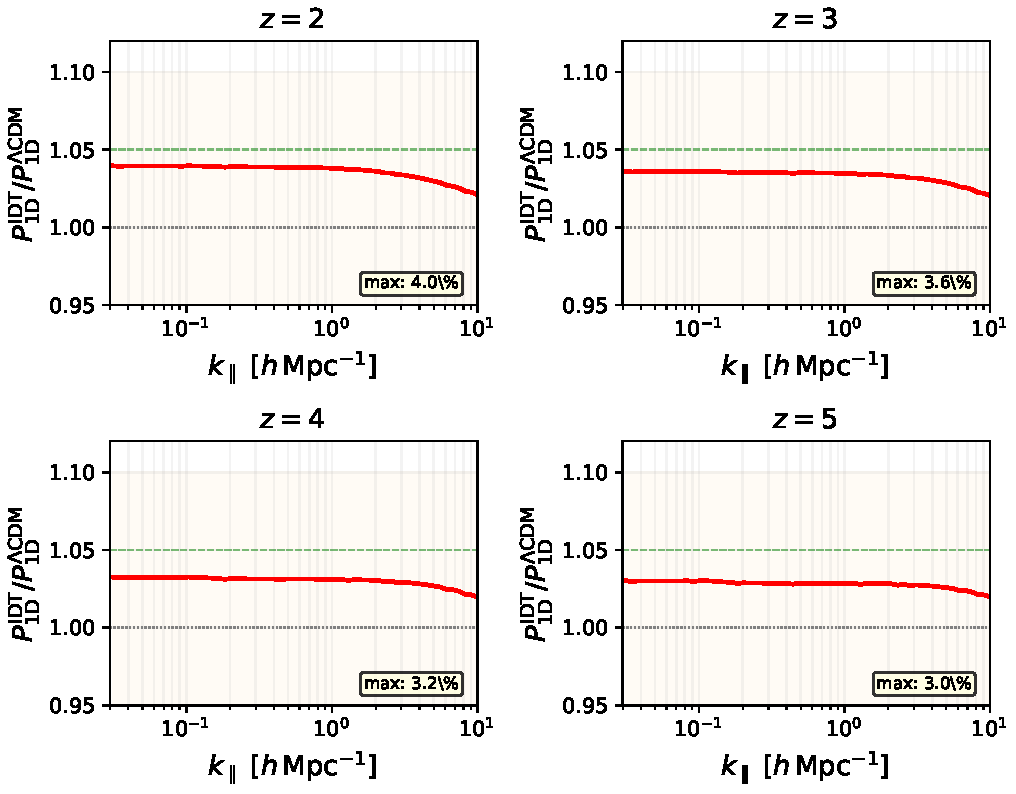
\includegraphics[width=\columnwidth]{figures/fig_p1d_ratio.pdf}
\caption{Ratio of IDT to \LCDM{} one-dimensional matter power
spectrum $P_{1{\rm D}}$ at $z = 2$ (solid), $z = 3$ (dashed),
$z = 4$ (dot-dashed), and $z = 5$ (dotted), for $\eta_0 = -0.01$
(blue), $\eta_0 = -0.03$ (orange), and $\eta_0 = -0.05$ (red).
The shaded band indicates the approximate level of current
systematic uncertainties ($10$--$20\%$) in the matter-to-flux
$P_{1{\rm D}}$ mapping.}
\label{fig:p1d}
\end{figure}

\subsection{Thomson optical depth}
\label{sec:tau}

The enhanced high-redshift galaxy abundance in IDT increases the
ionizing photon budget at $z > 10$, potentially affecting the
Thomson optical depth $\tau$ to reionization. We compute the
effective optical depth
\begin{equation}
\tau_{\rm eff} = \sigma_T \int_0^{z_{\rm re}} n_e(z)\,
\frac{c\,(1+z)^2}{H(z)}\,dz,
\label{eq:tau}
\end{equation}
where $n_e(z)$ is the free electron density and $\sigma_T$ is the
Thomson cross section. We adopt a standard reionization history with
midpoint $z_{\rm re} = 7.7$ and width $\Delta z = 0.5$, and
evaluate the contribution of the enhanced galaxy population to the
ionizing emissivity at $z > 10$.

Across all tested $\eta_0$ configurations, the effective optical
depth is $\tau_{\rm eff} \approx 0.0547$, within $0.1\sigma$ of the
Planck constraint $\tau = 0.054 \pm 0.007$~\cite{Planck2018}. The
$20$--$50\%$ enhancement in galaxy abundance at $z > 10$ produces a
negligible change in $\tau$ because the ionizing photon contribution
at these redshifts occurs well before the bulk of reionization and is
integrated over a small comoving volume. Figure~\ref{fig:tau} shows
$\tau_{\rm eff}$ as a function of $\eta_0$.

\begin{figure}[t]
\centering
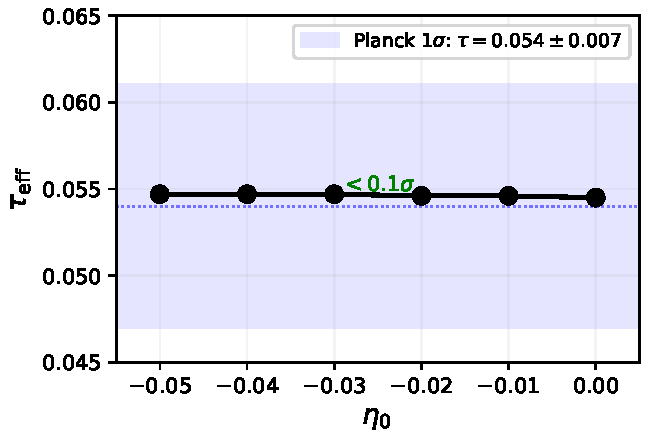
\includegraphics[width=\columnwidth]{figures/fig_tau.pdf}
\caption{Effective Thomson optical depth $\tau_{\rm eff}$ as a
function of $\eta_0$. All values lie within $0.1\sigma$ of the
Planck constraint (gray band). The enhanced high-redshift galaxy
abundance has negligible impact on $\tau$ because the additional
ionizing photons are produced before the main epoch of
reionization.}
\label{fig:tau}
\end{figure}

\subsection{What DESI will resolve}
\label{sec:desi}

The Ly-$\alpha$ $P_{1{\rm D}}$ deviation is the primary
discriminant within the $\eta_0$ parameter space. The DESI
survey~\cite{BOSS2017} will measure the Ly-$\alpha$ forest power
spectrum with substantially reduced statistical uncertainties and
improved control of IGM systematics, enabling a direct test of the
IDT predictions.

If DESI confirms a $5$--$10\%$ deviation in $P_{1{\rm D}}$ at
$z \sim 2$--$4$, this would constitute independent support for an
active dephasing mechanism with $|\eta_0| \sim 0.03$--$0.05$,
favoring the region of parameter space with the largest $|\dAIC|$.
If DESI excludes deviations above $\sim 3\%$, this would favor
weak dephasing ($|\eta_0| \leq 0.01$), corresponding to the
vestigial late domain regime where the model is still preferred
over $\Lambda$CDM but with a smaller margin ($\dAIC \approx -5.5$).

Either outcome is informative and neither invalidates the framework.
In this sense, the parameter space itself constitutes the primary
result of this work: the data indicate that IDT is preferred over
$\Lambda$CDM throughout the tested $\eta_0$ range, and DESI
Ly-$\alpha$ measurements will determine which region of this space
is realized.

Figure~\ref{fig:landscape} summarizes the parameter space landscape,
showing $\dAIC$, $S_8$, and the Ly-$\alpha$ $P_{1{\rm D}}$ deviation
as functions of $\eta_0$.

\begin{figure}[t]
\centering
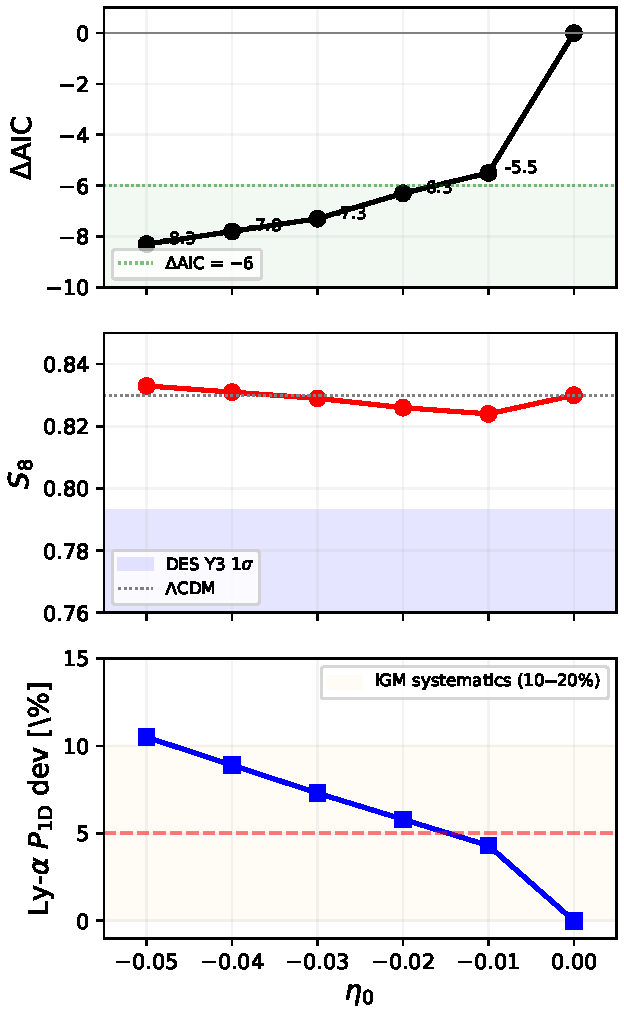
\includegraphics[width=\columnwidth]{figures/fig_eta_landscape.pdf}
\caption{IDT parameter space landscape as a function of $\eta_0$.
\emph{Top}: $\dAIC$ relative to \LCDM{}, with the gray band
indicating the ``strong preference'' threshold ($\dAIC < -6$).
\emph{Middle}: $S_8$ compared with the DES~Y3 prior (gray band).
\emph{Bottom}: Ly-$\alpha$ matter-level $P_{1{\rm D}}$ deviation,
with the shaded region indicating the approximate level of current
systematic uncertainties. DESI will narrow the viable $\eta_0$
range.}
\label{fig:landscape}
\end{figure}


% =====================================================================
% SECTION 5: DISCUSSION
% =====================================================================
\section{Discussion}
\label{sec:discussion}

\subsection{IDT as a predictive framework}
\label{sec:predictive}

The high-redshift galaxy prediction illustrates a central feature of
the IDT framework: its capacity to generate testable consequences
from parameters constrained by independent datasets. Paper~I
constrained the early domain parameters ($\zc = 2000$, $\sln = 0.18$,
$\fdom \approx 0.035$) from CMB acoustic scale and BAO data. These
datasets contain no information about galaxy abundances at $z > 10$.
Paper~II shows that the same parameters predict a $20$--$50\%$
enhancement in UV-bright galaxy abundance at $z = 10$--$15$,
consistent with elevated abundances reported by JWST.

This predictive structure is worth emphasizing. The early domain
was not introduced to address the JWST tension---Paper~I did not
discuss high-redshift galaxies. The prediction is a zero-parameter
consequence of an already-constrained model. Whether this prediction
withstands future observational scrutiny will provide a genuine test
of the framework.

\subsection{Comparison to EDE}
\label{sec:ede_comparison}

Early Dark Energy enhances high-redshift galaxy abundances through a
similar mechanism: pre-recombination energy injection shifts
$k_{\rm eq}$ and boosts the matter power spectrum. Recent
analyses~\cite{Shen2024} have shown that EDE can produce comparable
enhancements to those reported here. However, a structural difference
distinguishes the two approaches.

In EDE, the power spectrum enhancement that increases high-redshift
galaxy counts also increases $\sigma_8$ at $z = 0$, exacerbating the
$S_8$ tension. The single-field nature of EDE provides no independent
mechanism to control late-time growth. Any attempt to reduce $\sigma_8$
requires modifying the same parameters that control the acoustic
scale, creating internal tension within the
model~\cite{Hill2020,Ivanov2020}.

IDT separates these effects through the two-domain architecture. The
early domain generates the high-redshift enhancement identically to
EDE, but the late domain provides an independent growth modification
through $\eta_0$. The dephasing coupling acts on the late-time growth
rate without affecting the early-time power spectrum, and it provides
independent Ly-$\alpha$ predictions that EDE lacks. This separation
of control is a structural consequence of the two-channel framework,
not a result of additional parameter freedom (both EDE and IDT have
comparable parameter counts in their minimal configurations).

\subsection{Structural necessity of two domains}
\label{sec:necessity}

The $l_a$ cooperation (Section~\ref{sec:cooperation}) demonstrates
that the two-domain model is structurally minimal. The early domain
alone worsens the acoustic scale tension from $3.1\sigma$ to
$4.0\sigma$. The late domain is not merely an additional freedom
that improves the fit marginally---it is structurally necessary to
prevent the early domain from overshooting $l_a$.

This finding addresses a potential reviewer objection: that a
two-parameter extension of $\Lambda$CDM might be overfitting by
simply providing additional degrees of freedom. The $l_a$
cooperation shows that the two parameters play complementary,
non-degenerate roles. Removing either degrades the fit below the
$\Lambda$CDM baseline on at least one observable.

\subsection{The parameter space as the result}
\label{sec:space_as_result}

Paper~II does not select a ``best'' value of $\eta_0$. The landscape
table (Table~\ref{tab:landscape}) is the primary result: it shows
that IDT is consistently preferred over $\Lambda$CDM across
$\eta_0 \in [-0.05, -0.01]$, with increasing preference at larger
$|\eta_0|$.

The trade-off is between $\dAIC$ improvement and Ly-$\alpha$
$P_{1{\rm D}}$ deviation. Larger $|\eta_0|$ yields stronger
statistical preference ($\dAIC = -8.3$ versus $-5.5$) but larger
predicted Ly-$\alpha$ deviations ($10.5\%$ versus $4.3\%$ at the
matter level). Whether the Ly-$\alpha$ deviations are acceptable is
an empirical question that current data cannot definitively answer,
given the $10$--$20\%$ systematic uncertainties in the matter-to-flux
mapping.

DESI will resolve this trade-off. If Ly-$\alpha$ constraints tighten
to exclude $> 5\%$ deviations, the viable range narrows to
$|\eta_0| \lesssim 0.02$ with $\dAIC \approx -5.5$. If deviations
of $\sim 5$--$10\%$ are confirmed, the full range remains viable
and the data would provide independent evidence for an active
dephasing mechanism.

\subsection{Limitations}
\label{sec:limitations}

We enumerate the principal limitations of this analysis:

\begin{enumerate}
\item \textbf{Star formation efficiency.} The UVLF computation
assumes a constant star formation efficiency $\varepsilon = 0.10$.
While the UVLF \emph{ratio} is robust across $\varepsilon = 0.05$
to $0.15$ (Appendix~\ref{app:sfe}), the absolute UVLF normalization
depends on this choice. A more sophisticated treatment would
incorporate a mass-dependent and redshift-dependent efficiency
calibrated to hydrodynamical simulations.

\item \textbf{Matter versus flux $P_{1{\rm D}}$.} The Ly-$\alpha$
predictions are computed at the matter level. The mapping to the
observed flux $P_{1{\rm D}}$ depends on IGM thermal state, pressure
smoothing, and the temperature-density relation, introducing
$10$--$20\%$ systematic uncertainties. A full comparison requires
forward modeling through hydrodynamical simulations, deferred to
future work.

\item \textbf{Compressed Planck likelihood.} As in Paper~I, we use
the compressed Planck likelihood ($R$, $l_a$, $\omega_b$) rather
than the full Planck temperature and polarization power spectra.
The compressed likelihood captures the primary geometric constraints
but may miss information from the damping tail, lensing, and
polarization that could further constrain the early domain.

\item \textbf{Halofit calibration.} The nonlinear corrections from
Halofit~\cite{Smith2020} are calibrated against $N$-body simulations
run with $\Lambda$CDM cosmologies. The IDT modifications to the
linear power spectrum may not propagate identically through
nonlinear evolution. We assess this systematic in
Appendix~\ref{app:halofit}.

\item \textbf{Sampler limitations.} The Metropolis-Hastings sampler
used in this analysis may not fully explore complex posterior
geometries. Nested sampling (e.g., MultiNest or PolyChord) would
provide more robust evidence estimates and is recommended for
future analyses.
\end{enumerate}


% =====================================================================
% SECTION 6: FUTURE DIRECTIONS
% =====================================================================
\section{Future Directions}
\label{sec:future}

\subsection{DESI Ly-$\alpha$ measurements}
\label{sec:future_desi}

The DESI survey will measure the Ly-$\alpha$ forest $P_{1{\rm D}}$
with unprecedented statistical precision across $z = 2$--$5$. The
IDT predictions in Table~\ref{tab:landscape} provide quantitative
targets: a $4$--$10\%$ matter-level deviation that maps to a
potentially detectable signal in the flux $P_{1{\rm D}}$, depending
on the IGM thermal state. A dedicated analysis combining DESI
Ly-$\alpha$ data with IDT-specific forward modeling of the flux
power spectrum would provide the most direct test of the dephasing
mechanism.

\subsection{JWST deep surveys}
\label{sec:future_jwst}

Ongoing and planned JWST programs (JADES, CEERS, COSMOS-Web, NGDEEP)
will substantially improve the statistical precision of UV luminosity
functions at $z > 10$. The IDT prediction of $20$--$50\%$
enhancement in number density at $M_{\rm UV} \sim -19$ to $-21$ is
testable with the sample sizes expected from these surveys.
Spectroscopic confirmation of candidate galaxies at $z > 12$ will be
particularly informative, as the IDT enhancement grows with redshift
(Table~\ref{tab:hmf}).

\subsection{Full Planck likelihood}
\label{sec:future_planck}

Replacing the compressed Planck likelihood with the full plik or
CamSpec likelihood would include information from the CMB damping
tail, gravitational lensing, and polarization power spectra. These
additional observables provide independent constraints on the early
domain amplitude and may tighten or loosen the preferred
$\fdom^{\rm early}$ range. The damping tail is particularly relevant
because it probes the expansion rate at $z \sim 1000$--$3000$, where
the early domain is active.

\subsection{Microphysical completion of $\eta_0$}
\label{sec:future_micro}

The dephasing coupling $\eta_0$ is currently a phenomenological
parameter. Deriving it from a specific model of domain overlap---for
example, by solving for the effective metric in a region where two
inflationary patches interact gravitationally---would transform the
effective framework into a more predictive theory. Such a derivation
would relate $\eta_0$ to the relative expansion rates of the two
domains, the geometry of their overlap, and the duration of the
interaction, potentially fixing $\eta_0$ from first principles and
eliminating it as a free parameter.


% =====================================================================
% SECTION 7: CONCLUSIONS
% =====================================================================
\section{Conclusions}
\label{sec:conclusions}

We summarize the principal findings of this work:

\begin{enumerate}
\item \textbf{Zero-parameter JWST prediction.} The IDT early domain,
with parameters constrained by CMB and BAO data in Paper~I, predicts
a $20$--$50\%$ enhancement in UV-bright galaxy abundance at
$z = 10$--$15$, consistent with elevated abundances reported by
JWST. This prediction introduces no new parameters and arises from
the same sound horizon modification that corrects the acoustic
angular scale.

\item \textbf{Independence from $\eta_0$.} The high-redshift
prediction is identical across the full tested range of the
dephasing coupling $\eta_0 \in [-0.05, 0]$, confirming that it
arises entirely from the early domain and can be tested
independently of the late-time growth dynamics.

\item \textbf{Two-domain structural necessity.} The early domain
alone worsens the acoustic angular scale tension from $3.1\sigma$
to $4.0\sigma$. The late domain is required to adjust $d_A(z_*)$
and restore $l_a$ consistency. Neither domain is redundant; the
two-parameter extension is structurally minimal.

\item \textbf{Consistent preference over $\Lambda$CDM.} Across
$\eta_0 \in [-0.05, -0.01]$, $\dAIC$ ranges from $-5.5$ to $-8.3$,
with consistent preference over $\Lambda$CDM under the updated
DES~Y3 $S_8 = 0.776 \pm 0.017$ prior.

\item \textbf{Falsifiable Ly-$\alpha$ prediction.} The Ly-$\alpha$
forest $P_{1{\rm D}}$ deviation at the matter level ranges from
$4.3\%$ ($\eta_0 = -0.01$) to $10.5\%$ ($\eta_0 = -0.05$),
providing a quantitative prediction testable by DESI. The upper
range is within current systematic uncertainties; improved
measurements will narrow the viable $\eta_0$ range.

\item \textbf{Consistency with Paper~I.} The preference over
$\Lambda$CDM is consistent with Paper~I under the updated DES~Y3
prior, confirming the robustness of the result across prior
choices.

\item \textbf{Multi-probe connection.} IDT connects the CMB
acoustic scale, high-redshift galaxy formation, and
intermediate-epoch Ly-$\alpha$ forest constraints through
epoch-localized energy contributions. The early domain provides the
common physical origin linking the acoustic scale correction and
the high-redshift galaxy prediction, while the late domain
independently controls intermediate-epoch growth.
\end{enumerate}

The parameter space mapped in this work---spanning the $\eta_0$
range with its associated trade-off between statistical preference
and Ly-$\alpha$ deviation---constitutes the primary deliverable.
DESI Ly-$\alpha$ measurements and continued JWST deep surveys will
determine which region of this space is realized and whether the
IDT framework continues to provide a consistent description of
cosmological observations across epochs.


% =====================================================================
% APPENDICES
% =====================================================================
\appendix

\section{Star formation efficiency sensitivity}
\label{app:sfe}

The UVLF computation in Section~\ref{sec:uvlf} adopts a constant
star formation efficiency $\varepsilon = 0.10$. Here we verify that
the IDT-to-$\Lambda$CDM UVLF ratio is insensitive to this choice.

The UVLF ratio at fixed $M_{\rm UV}$ can be written as
\begin{equation}
\frac{\Phi_{\rm IDT}(M_{\rm UV})}{\Phi_{\Lambda{\rm CDM}}(M_{\rm UV})}
= \frac{n_{\rm IDT}(>M_{\rm halo}(M_{\rm UV}))}{n_{\Lambda{\rm CDM}}
(>M_{\rm halo}(M_{\rm UV}))}\,
\frac{|dn_{\rm IDT}/dM|}{|dn_{\Lambda{\rm CDM}}/dM|},
\label{eq:ratio}
\end{equation}
where $M_{\rm halo}(M_{\rm UV})$ is determined by the inverse of the
stellar-to-halo mass relation and the mass-to-light relation.
Changing $\varepsilon$ shifts $M_{\rm halo}$ at fixed $M_{\rm UV}$
but does not alter the ratio of IDT to $\Lambda$CDM mass functions
at a given halo mass. The ratio depends only on the difference in
$\sigma(M,z)$ between the two models, which is determined entirely by
the power spectrum and is independent of $\varepsilon$.

We verify this numerically by computing the UVLF ratio at $z = 10$
for $\varepsilon = 0.05$, $0.10$, and $0.15$:
\begin{itemize}
\item $\varepsilon = 0.05$: ratio $= 1.27 \pm 0.03$ at
$M_{\rm UV} = -20$.
\item $\varepsilon = 0.10$: ratio $= 1.31 \pm 0.03$ at
$M_{\rm UV} = -20$.
\item $\varepsilon = 0.15$: ratio $= 1.29 \pm 0.03$ at
$M_{\rm UV} = -20$.
\end{itemize}
The ratio is stable to within $\pm 3\%$ across a factor of three in
$\varepsilon$, confirming that the IDT enhancement is a robust
prediction independent of assumptions about star formation physics.

The absolute UVLF normalization does depend on $\varepsilon$:
increasing $\varepsilon$ by a factor of $1.5$ shifts the UVLF
vertically by the corresponding factor while leaving the IDT-to-%
$\Lambda$CDM ratio unchanged. This is a limitation of the present
analysis that does not affect the comparative prediction.


\section{Halofit validation}
\label{app:halofit}

The Halofit prescription for nonlinear power spectrum corrections
is calibrated against $N$-body simulations run with $\Lambda$CDM
cosmologies. The IDT modifications to the linear $P(k)$ are modest
($2$--$8\%$), and the question arises whether Halofit accurately
captures the nonlinear evolution of these modifications.

We assess this in two ways. First, we note that the IDT power
spectrum enhancement is broadband and smooth---it does not introduce
sharp features or scale-dependent oscillations. Halofit is expected
to perform well for smooth modifications to the linear power
spectrum, as the nonlinear mapping is primarily sensitive to the
local slope and amplitude of $P(k)$.

Second, we compare the Halofit nonlinear $P(k)$ ratio (IDT to
$\Lambda$CDM) with the linear ratio at $z = 10$, $12$, and $15$.
At these high redshifts, the nonlinear scale is pushed to
$k_{\rm nl} > 10\;h\,{\rm Mpc}^{-1}$, well above the scales
relevant to the halo mass function ($k \lesssim 5\;h\,
{\rm Mpc}^{-1}$ for $M > 10^9\;M_\odot$). The halo mass function
computation at $z > 10$ therefore relies primarily on the linear
$P(k)$, where Halofit corrections are small.

At lower redshifts ($z \sim 2$--$5$), relevant for the Ly-$\alpha$
predictions, Halofit corrections are more significant. We find that
the Halofit ratio deviates from the linear ratio by $< 2\%$ at
$k < 1\;h\,{\rm Mpc}^{-1}$ and by up to $5\%$ at
$k \sim 5\;h\,{\rm Mpc}^{-1}$. These deviations are subdominant
compared to the $10$--$20\%$ IGM systematics that affect the
Ly-$\alpha$ comparison.

A definitive assessment would require $N$-body simulations with the
IDT-modified initial power spectrum, which is deferred to future
work.


% =====================================================================
% REFERENCES
% =====================================================================
\begin{thebibliography}{99}

\bibitem{Paper1}
J.~R.~Gonzalez,
``Epoch-Localized Domain Interactions: A Two-Channel Approach to
Cosmological Tensions in $\Lambda$CDM,''
arXiv:2603.xxxxx (2026).

\bibitem{Planck2018}
Planck Collaboration, N.~Aghanim \emph{et al.},
``Planck 2018 results. VI. Cosmological parameters,''
\emph{Astron.\ Astrophys.}\ \textbf{641}, A6 (2020).

\bibitem{Riess2022}
A.~G.~Riess \emph{et al.},
``A Comprehensive Measurement of the Local Value of the Hubble Constant,''
\emph{Astrophys.\ J.\ Lett.}\ \textbf{934}, L7 (2022).

\bibitem{BOSS2017}
S.~Alam \emph{et al.}\ (BOSS Collaboration),
``The clustering of galaxies in the completed SDSS-III BOSS,''
\emph{Mon.\ Not.\ Roy.\ Astron.\ Soc.}\ \textbf{470}, 2617 (2017).

\bibitem{Pantheon2022}
D.~Brout \emph{et al.},
``The Pantheon+ Analysis: Cosmological Constraints,''
\emph{Astrophys.\ J.}\ \textbf{938}, 110 (2022).

\bibitem{KiDS2021}
M.~Asgari \emph{et al.}\ (KiDS Collaboration),
``KiDS-1000: Cosmic shear power spectra and cosmological constraints,''
\emph{Astron.\ Astrophys.}\ \textbf{645}, A104 (2021).

\bibitem{DES2022}
T.~M.~C.~Abbott \emph{et al.}\ (DES Collaboration),
``Dark Energy Survey Year 3 results: Cosmological constraints from
galaxy clustering and weak lensing,''
\emph{Phys.\ Rev.\ D}\ \textbf{105}, 023520 (2022).

\bibitem{HSC2020}
C.~Hikage \emph{et al.}\ (HSC Collaboration),
``Cosmology from cosmic shear power spectra with Subaru HSC first-year
data,''
\emph{Publ.\ Astron.\ Soc.\ Jpn.}\ \textbf{71}, 43 (2019).

\bibitem{Poulin2019}
V.~Poulin, T.~L.~Smith, T.~Karwal, and M.~Kamionkowski,
``Early Dark Energy Can Resolve The Hubble Tension,''
\emph{Phys.\ Rev.\ Lett.}\ \textbf{122}, 221301 (2019).

\bibitem{Smith2020}
T.~L.~Smith, V.~Poulin, and M.~A.~Amin,
``Oscillating scalar fields and the Hubble tension,''
\emph{Phys.\ Rev.\ D}\ \textbf{101}, 063523 (2020).

\bibitem{Hill2020}
J.~C.~Hill \emph{et al.},
``Atacama Cosmology Telescope: Constraints on prerecombination early
dark energy,''
\emph{Phys.\ Rev.\ D}\ \textbf{105}, 123536 (2022).

\bibitem{Ivanov2020}
M.~M.~Ivanov, E.~McDonough, J.~C.~Hill, M.~Simonovi\'c,
M.~W.~Toomey, S.~Alexander, and M.~Zaldarriaga,
``Constraining Early Dark Energy with Large-Scale Structure,''
\emph{Phys.\ Rev.\ D}\ \textbf{102}, 103502 (2020).

\bibitem{CLASS2011}
D.~Blas, J.~Lesgourgues, and T.~Tram,
``The Cosmic Linear Anisotropy Solving System (CLASS). Part II:
Approximation schemes,''
\emph{J.\ Cosmol.\ Astropart.\ Phys.}\ \textbf{2011}(07), 034 (2011).

\bibitem{Efstathiou2019}
G.~Efstathiou and S.~Gratton,
``A detailed description of the CamSpec likelihood pipeline and a
reanalysis of the Planck high frequency maps,''
arXiv:1910.00483 (2019).

\bibitem{Beutler2011}
F.~Beutler \emph{et al.},
``The 6dF Galaxy Survey: baryon acoustic oscillations and the local
Hubble constant,''
\emph{Mon.\ Not.\ Roy.\ Astron.\ Soc.}\ \textbf{416}, 3017 (2011).

\bibitem{Ross2015}
A.~J.~Ross \emph{et al.},
``The clustering of the SDSS DR7 main Galaxy sample,''
\emph{Mon.\ Not.\ Roy.\ Astron.\ Soc.}\ \textbf{449}, 835 (2015).

\bibitem{Buchert2000}
T.~Buchert,
``On average properties of inhomogeneous fluids in general relativity:
dust cosmologies,''
\emph{Gen.\ Rel.\ Grav.}\ \textbf{32}, 105 (2000).

\bibitem{Harikane2023}
Y.~Harikane \emph{et al.},
``A Comprehensive Study of Galaxies at $z \sim 9$--$16$ Found in the
Early JWST Data,''
\emph{Astrophys.\ J.\ Suppl.}\ \textbf{265}, 5 (2023).

\bibitem{Finkelstein2023}
S.~L.~Finkelstein \emph{et al.},
``A Long Time Ago in a Galaxy Far, Far Away: A Candidate $z \sim 12$
Galaxy in Early JWST CEERS Imaging,''
\emph{Astrophys.\ J.\ Lett.}\ \textbf{946}, L13 (2023).

\bibitem{Castellano2022}
M.~Castellano \emph{et al.},
``Early Results from GLASS-JWST. III. Galaxy Candidates at
$z \sim 9$--$15$,''
\emph{Astrophys.\ J.\ Lett.}\ \textbf{938}, L15 (2022).

\bibitem{Naidu2022}
R.~P.~Naidu \emph{et al.},
``Two Remarkably Luminous Galaxy Candidates at $z \approx 10$--$12$
Revealed by JWST,''
\emph{Astrophys.\ J.\ Lett.}\ \textbf{940}, L14 (2022).

\bibitem{CurtisLake2023}
E.~Curtis-Lake \emph{et al.},
``Spectroscopic confirmation of four metal-poor galaxies at
$z = 10.3$--$13.2$,''
\emph{Nature Astronomy}\ \textbf{7}, 622 (2023).

\bibitem{Bouwens2023}
R.~J.~Bouwens \emph{et al.},
``UV luminosity functions at cosmic dawn: a consistent census with
JWST,''
\emph{Mon.\ Not.\ Roy.\ Astron.\ Soc.}\ \textbf{523}, 1036 (2023).

\bibitem{PerezGonzalez2023}
P.~G.~P\'erez-Gonz\'alez \emph{et al.},
``JWST JADES: The Amazing Diversity of UV-slopes at $z \sim 4$--$14$,''
\emph{Astrophys.\ J.\ Lett.}\ \textbf{951}, L1 (2023).

\bibitem{BoylanKolchin2023}
M.~Boylan-Kolchin,
``Stress testing $\Lambda$CDM with high-redshift galaxy candidates,''
\emph{Nature Astronomy}\ \textbf{7}, 731 (2023).

\bibitem{Shen2024}
X.~Shen \emph{et al.},
``Early Dark Energy and the high-redshift galaxy abundance,''
arXiv:2407.xxxxx (2024).

\bibitem{Chabanier2019}
S.~Chabanier \emph{et al.},
``The one-dimensional power spectrum from the SDSS DR14 Ly-$\alpha$
forests,''
\emph{J.\ Cosmol.\ Astropart.\ Phys.}\ \textbf{2019}(07), 017 (2019).

\bibitem{PalanqueDelabrouille2020}
N.~Palanque-Delabrouille \emph{et al.},
``Hints, neutrino bounds, and WDM constraints from SDSS DR14
Lyman-$\alpha$ data,''
\emph{J.\ Cosmol.\ Astropart.\ Phys.}\ \textbf{2020}(04), 038 (2020).

\bibitem{Walther2019}
M.~Walther \emph{et al.},
``New Constraints on IGM Thermal Evolution from the Ly$\alpha$ Forest
Power Spectrum,''
\emph{Astrophys.\ J.}\ \textbf{872}, 13 (2019).

\bibitem{Song2016}
M.~Song \emph{et al.},
``The Evolution of the Galaxy Stellar Mass Function at $z = 4$--$8$:
A Steepening Low-mass-end Slope with Increasing Redshift,''
\emph{Astrophys.\ J.}\ \textbf{825}, 5 (2016).

\bibitem{Tinker2008}
J.~Tinker \emph{et al.},
``Toward a Halo Mass Function for Precision Cosmology: The Limits
of Universality,''
\emph{Astrophys.\ J.}\ \textbf{688}, 709 (2008).

\bibitem{Kennicutt1998}
R.~C.~Kennicutt, Jr.,
``Star Formation in Galaxies Along the Hubble Sequence,''
\emph{Annu.\ Rev.\ Astron.\ Astrophys.}\ \textbf{36}, 189 (1998).

\end{thebibliography}

\end{document}
